\subsection{Décodeur 7seg}
\begin{figure}[ht]
    \centering
    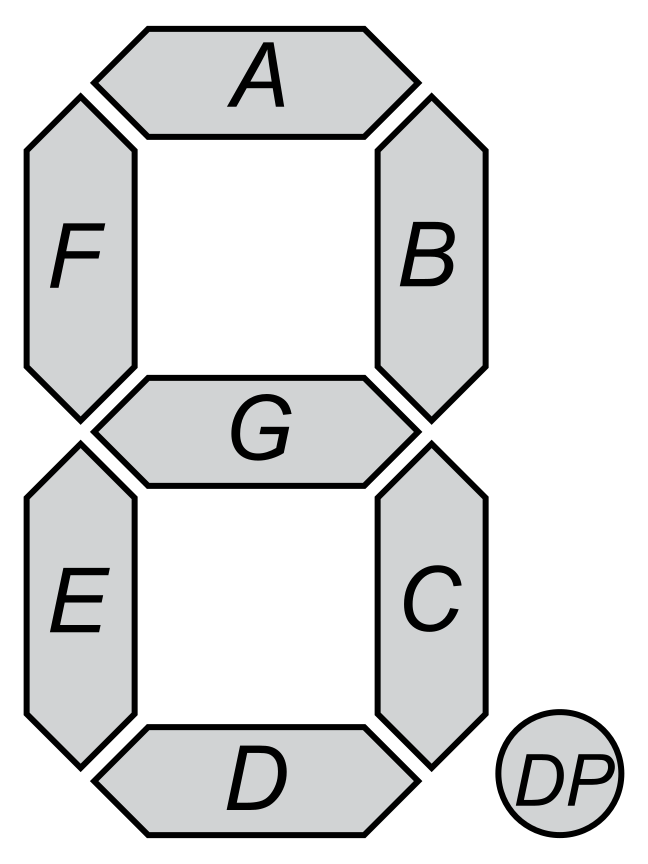
\includegraphics[scale = 0.1]{img/SevenSegDisplay.png}
    \caption{Segments d'un afficheur}
\end{figure}

Un afficheur sept segments est utilisé pour afficher des informations vers un utilisateur en allumant une partie des segments. Par exemple, pour afficher le chiffre \textit{2}, on allume les segments \textit{A, B, D, E, G}.

\medskip

- Décrire la table de vérité de l'afficheur sept segments pour les chiffres allant de \textbf{$0_d$ à $15_d$ en hexadécimal}

\medskip

- Décrire l'entité et l'architecture de votre table de vérité en VHDL.

\medskip

- Simuler et vérifier le bon comportement de votre table de vérité

\medskip

- Connecter les entrées de votre décodeur sept segments aux switchs (SW$x$) et les sorties aux afficheurs sept segments (HEX$x$) de la carte DE2. Tester et vérifier le bon fonctionnement.
